\documentclass[tikz,border=10pt]{standalone}
\usepackage{tikz}
\usepackage{tikz-cd}
\usetikzlibrary{arrows,automata,shapes,positioning,decorations.pathmorphing}
% \tikzset{->,>=stealth',auto}
\tikzset{->,auto}
\tikzset{>={Latex[width=2mm,length=2mm]}}
\tikzset{state/.style={shape=circle, draw, fill=white, initial text=,
    inner sep=.5mm, minimum size=2mm}}
\tikzset{state with output/.style={shape=rectangle split, rectangle
    split parts=2, draw, fill=white,
    initial text=, inner sep=1mm}}
\begin{document}
 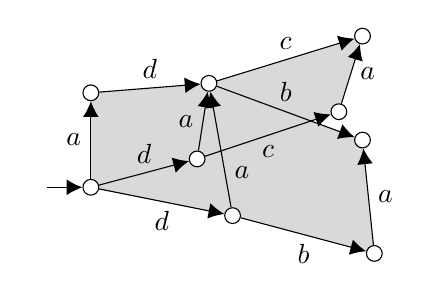
\begin{tikzpicture}[x=1.5cm, y=1.2cm]
    \coordinate (00') at (0,0);
    \coordinate (10a') at (1.2,-.3);
    \coordinate (20a') at (2.4,-.7);
    \coordinate (10b') at (.9,.3);
    \coordinate (20b') at (2.1,.8);
    \coordinate (01') at (0,1);
    \coordinate (11') at (1,1.1);
    \coordinate (21a') at (2.3,.5);
    \coordinate (21b') at (2.3,1.6);

    \fill[gray!30] (00') -- (10a') -- (20a') -- (21a') -- (11') --
    (01') -- (00');
    \fill[gray!30] (00') -- (10b') -- (20b') -- (21b') -- (11') --
    (01') -- (00');

    \node[state, initial] (00) at (00') {};
    \foreach \a in {10a,20a,10b,20b,01,11,21a,21b}
    \node[state] (\a) at (\a') {};

    \path (00) edge node[below] {$d$} (10a);
    \path (10a) edge node[below] {$b$} (20a);
    \path (00) edge node[above] {$d$} (10b);
    \path (10b) edge node[below] {$c$} (20b);
    \path (01) edge node[above] {$d$} (11);
    \path (11) edge node[above] {$b$} (21a);
    \path (11) edge node[above] {$c$} (21b);
    \path (00) edge node[left] {$a$} (01);
    \path (10a) edge node[right, pos=.3] {$a$} (11);
    \path (10b) edge node[left] {$a$} (11);
    \path (20a) edge node[right] {$a$} (21a);
    \path (20b) edge node[right] {$a$} (21b);
  \end{tikzpicture}
\end{document}